\documentclass{beamer} 
%
% Choose how your presentation looks.
%
% For more themes, color themes and font themes, see:
% http://deic.uab.es/~iblanes/beamer_gallery/index_by_theme.html
%
\mode<presentation>
{
  \usetheme{default}      % or try Darmstadt, Madrid, Warsaw, ...
  \usecolortheme{default} % or try albatross, beaver, crane, ...
  \usefonttheme{default}  % or try serif, structurebold, ...
  \setbeamertemplate{navigation symbols}{}
  \setbeamertemplate{caption}[numbered]
} 

\usepackage[english]{babel}
\usepackage[utf8x]{inputenc}
\usepackage{amsmath,amsthm,amssymb,amsfonts}
\usepackage[ruled,longend]{algorithm2e}
\newtheorem*{dfn}{Definition}
\newtheorem{thm}{Theorem}[subsection]
 \renewcommand{\thethm}{\arabic{thm}}
%\newtheorem{lemma}{Lemma}
\title[Introduction]{Statistics Learning Theory:Logistic Regression I computational aspect}
\author{}
\institute{}
\date{2019.02.23}

\begin{document}

\begin{frame}
  \titlepage
\end{frame}

% Uncomment these lines for an automatically generated outline.
%\begin{frame}{Outline}
%  \tableofcontents
%\end{frame}

\section{Logistic Regression}
\begin{frame}{Logistic Regression:Sigmoid Function}
	In this week slide, we will introduce the implementation of Logistic regression and related property. \\
	To understand the method of logistic regression, we first introduce the sigmoid function. That is, the function $\sigma_{sig}:R \rightarrow [0,1]$ over the class of linear functions $L_d$ such that
	\[\sigma_{sig}(z) = \frac{1}{1+exp(-z)}\]
	The hypothesis class becomes
\[\mathcal{H} = \sigma_{sig} \circ L_d = \{x \rightarrow \sigma_{sig}(\langle w,x \rangle)): w \in R^d\}\]
\end{frame}
\begin{frame}{Logistic Regression:Loss function}
	Given the classifier $h_{w}(x)$, we should define how bad it is to predict some $h_w(x) \in [0,1]$ given that the true label is $y \in \{1,-1\}$ \\
	Therefore, we would like that $h_w(x)$ would be large if $y=1$ and that $1-h_w(x)$ would be large if $y=-1$. Since
	\[1 - h_w(x) = \frac{1}{1+exp(\langle w,x \rangle)}\]
	Therefore, any resonable loss function would increase monotonically with $\frac{1}{1+exp( y \langle w,x \rangle)}$
\end{frame}
\begin{frame}{Logistic Regression:Loss function}
	We can choose the log function, that is the loss function
	\[l(h_w,(x,y)) = \log (1+exp( -y \langle w,x \rangle)\]
	The ERM problem associated with logistic regression is 
	\[arg\min_{w \in R^d} \frac{1}{m} \sum^m_{i=1} \log(1+exp( -y \langle w,x \rangle)\]
\end{frame}
\begin{frame}{Logistic Regression: Remark}
	\begin{enumerate}
		\item logistic loss function is convex function, the optimization can be solved efficienyly
		\item The ERM problem associated with logistic regress is identical to the problem of finding a maximimum Likelihood Estimator.
		\item One of the efficient algorithm is stochastic gradient descent
	\end{enumerate}
\end{frame}
\begin{frame}
	 \begin{block}{Sigmoid function}
		 % Your image included here
		 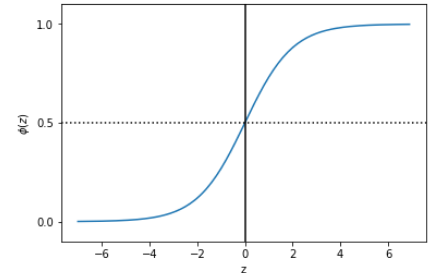
\includegraphics[width=\textwidth]{Sigmoid.png}
	\end{block}
\end{frame}
\begin{frame}{Gradient Descent:Motivation}
	The Taylor approximation tells us that 
	\[f(u) \approx f(w) + \langle u-w,\nabla f(w) \rangle \]
	Therefore, given the point $w^{(t)}$, we can update the the next point by minimizing the approximation of $f(u)$, however, when $u$ is far away from $w^{t}$, the approximation might become loose. Hence, we jointly minimize the distance between $u$ and $w^{(t)}$ and approximation around $w^{(t)}$. That is
	\[w^{(t+1)} = arg\min_{u} \frac{1}{2} |u-w^{(t)}|^2 + \eta(f(w^{(t)}) + \langle u - w^{(t)}, \nabla f(w^{(t)}) \rangle)\]
\end{frame}
\begin{frame}{Gradient Gescent:Motivation}
	Taking the derivative with respect to $u$, we can obtain the following:
	\[w^{(t+1)} = w^{(t)} - \eta \nabla f(w^{(t)})\]
	The algorithm will update the value in the direction of the greatest rate of increase of $f$ around $w^{(t)}$, $\eta $ can be thought as learning rate, the rate we believe the approximation part.
\end{frame}
\begin{frame}{Analysis of GD for Convex-Lipschitz Functions}
	In the GD algorithm, we assume the output is $\bar{w} = \frac{1}{T} \sum^T_{t=1} w^{(t)}$ and denote $w^*$ as the minimizer of $f(w)$. By the convexity and the definition of $\bar{w}$, we have 
\[f(\bar{w}) - f(w^*) = f(\frac{1}{T} \sum^T_{t=1} w^{(t)}) - f(w^*)\]
	\[	\leq \frac{1}{T} \sum^T_{t=1} (f(w^{(t)}) - f(w^*)\]
		\[= \frac{1}{T} \sum^T_{t=1} (f(w^{(t)}) - f(w^*)) \]
		because of the convexity of $f$, we have that 	
		\[f(w^{(t)}) - f(w^*) \leq \langle w^{(t)} - w^*, \nabla f(w^{(t)}) \rangle\]
Therefore
\[f(\bar{w}) - f(w^*) \leq \frac{1}{T} \sum^T_{t=1} \langle w^{(t)} - w^*, \nabla f(w^{(t)}) \rangle\]
\end{frame}
\begin{frame}{Analysis of GD for Convex-Lipschitz Functions}
	To estimate the converge rate of GD algorithm, we claim the following lemma
	\begin{thm}
		Let $v_1, \cdots,v_T$ be an arbitrary sequence of vectors. Any algorithm with an initialization $w^{(1)}=0$ and an update rule of the form
		\[w^{(t+1)} = w^{(t)} - \eta v_t\]
		satisfies
\[\sum^T_{t=1} \langle w^{(t)} - w^*, v_t \rangle \leq \frac{|w^*|^2}{2 \eta} + \frac{\eta}{2} \sum^T_{t=1} |v_t|^2\]
In particular, if $|v_t| \leq \rho$ and $|w^*| \leq B$ then we set $\eta = \sqrt{\frac{B^2}{\rho^2 T}}$ then
\[\frac{1}{T} \sum^T_{t=1} \langle w^{(t)} - w^*,v_t \rangle \leq \frac{B \rho}{\sqrt{T}}\]
	\end{thm}
\end{frame}
\begin{frame}{Analysis of GD for Convex-Lipschitz Functions}
	Using albegraic manipulations, we have 
	\[\langle w^{(t)} - w^*,v_t \rangle = \frac{1}{\eta} \langle w^{(t)} - w^*, \eta v_t \rangle\]
	\[= \frac{1}{2 \eta} (-|w^{(t)} - w^* - \eta v_t |^2 + |w^{(t)} - w^*|^2 + \eta^2 |v_t|^2)\]
	\[= \frac{1}{2\eta} ( - |w^{(t+1)} - w^*|^2 + |w^{(t)} - w^*|^2) + \frac{\eta}{2} |v_t|^2\]
	Summing the equality over $t$, we have 
	\[\sum^T_{t=1} \langle w^{(t)} - w^*,v_t \rangle = \frac{1}{2 \eta} \sum^T_{t=1} ( - |w^{(t+1)} - w^*|^2 + |w^{(t)} - w^*|^2) + \frac{\eta}{2} |v_t|^2\]
\end{frame}
\begin{frame}{Analysis of GD for Convex-Lipschitz Functions}
The first part is a telescopic sum equal to 
\[|w^{(1)} - w^*|^2 - |w^{(T+1)} - w^*|^2\]
Therefore
\[sum^T_{t=1} \langle w^{(t)} - w^*,v_t \rangle = \frac{1}{2 \eta} (|w^{(1)} - w^*|^2 - |w^{(T+1)} - w^*|^2) + \frac{\eta}{2} \sum^T_{t=1} |v_t|^2\]
\[\leq \frac{1}{2 \eta} |w^{(1)} - w^*|^2 + \frac{\eta}{2} \sum^T_{t=1} |v_t|^2\]
\[= \frac{1}{2 \eta} |w^*|^2 + \frac{\eta}{2} \sum^T_{t=1} |v_t|^2\]
\end{frame}
\begin{frame}{Gereralized:Subgradients}
	We want to generalize to non-differentable functions. To do this, we use subgradients instead. Here, we recall the definition of subgradient.
	\begin{dfn}
		A vector $v$ that satisfies 
		\[\forall u \in S, \ \ f(u) \geq f(w) + \langle u-w,v \rangle\]
		is called a subgradient of $f$ at w. The set of subgradients of $f$ at w is called  the differential set and denoted $\partial f(w)$. Note that if $f$ is convex, such v must exist.
	\end{dfn}
\end{frame}
\begin{frame}{Stochastic Gradient Descent}
	\begin{algorithm}[H]
		$Input: \gets \text{Scalar} \ \  \eta>0, \text{integer} T>0$ \;
		$Initialize: \gets w^{(1)} = (0,0,\cdots,0)$\;
		\For{$t = 1,2, \cdots T$}
		{    choose $v_t$ at random from a distribution such that $E[v_t|w^{(t)}] \in \partial f(w^{(t)})$
			\\
			 update			$w^{(t+1)} = w^{(t)} - \eta v_t$\;
							}
	$Output: \bar{w} = \frac{1}{T} \sum^{T}_{t=1} w^{(t)}$
	\caption{Stochastic Gradient Descent(SGD)}
	\end{algorithm}
\end{frame}
\begin{frame}{Stochastic Gradient Descent:theorem}
	\begin{thm}	
		Let $B,\rho>0$. Let $f$ be a convex function and let $w^* \in arg\min_{w:|w| \leq B} f(w)$. Assume that SGD is run for $T$ iterations with $\eta = \sqrt{\frac{B^2}{\rho^2 T}}$. Assume also that for all $t$, $|v_t| \leq \rho$ with probability 1. Then,
		\[E[f(\bar{w})] - f(w^*) \leq \frac{b \rho}{\sqrt{T}}\]
	\end{thm}
\end{frame}
\begin{frame}{Gradient Descent}
	\begin{algorithm}[H]
		$Goal:Find \ \ arg\min_x f(x)$ \\
		$Input: \gets \text{Scalar} \ \  \eta>0, \text{integer} T>0$ \;
		$Initialize: \gets w^{(1)} = (0,0,\cdots,0)$\;
		\For{$t = 1,2, \cdots T$}
		{   
			update			$w^{(t+1)} = w^{(t)} - \eta \nabla f(w^t)$\;
							}
	$Output: \bar{w} = \frac{1}{T} \sum^{T}_{t=1} w^{(t)}$
	\caption{Gradient Descent(GD)}
	\end{algorithm}
\end{frame}
\end{document}
